\section{Numerical and Experimental Evaluation} \label{sec:experiments}

The goal of this section is to evaluate the proposed control methods. To this end, we define the following metrics:
\begin{itemize}
    \item \sout{\textit{Average stage cost}: this performance metric is computed by averaging the stage cost evaluated at each time step. Task duration and cost scheduling is kept fixed among all the experiments.}  
    \item \textit{Cumulative constraints violation}: as each barrier function is, by definition, negative outside of the safe set, we define the following metric as a proxy for the size of the constraint violation along the duration of an experiment:
    \begin{equation*}
        \Delta^{i}_{tot} = \sum\limits_{k=0}^{K_{exp}} \max(0, -h^i(\vect{x}_{k \Delta t})),
    \end{equation*}
    referring to the $i$th ZBF, where $K_{exp} = \lfloor T_{exp} / \Delta t \rfloor$.
    \item \textit{Average interaction wrench}: average wrench which is exerted on the environment during the execution of the task.
    \item \textit{Dissipated power}: during an ideal interaction with an articulated object, power is minimally dissipated. Therefore, we use the dissipated power as an efficiency metric:
    \begin{equation}
        P_{diss} = \sum\limits_{0}^{T_{exp}} -\command^T \boldsymbol{\tau}_{ext}.
    \end{equation}
\end{itemize}
The simulation experiments are conducted on a dynamic manipulator model as described by \eqref{eq:eom}. The manipulation tasks consist of maneuvering different articulated objects: a \textit{shelf}, a \textit{dishwasher}, a \textit{microwave} and a \textit{drawer} as shown in \fig\ref{fig:object_manipulation}. They differ in type and orientation of the joint. The \textit{shelf} and \textit{microwave} have a vertical revolute joint, the \textit{dishwasher} has a horizontal revolute joint, while the \textit{drawer} has a horizontal prismatic joint.
  
\begin{figure}[t]
\centering
  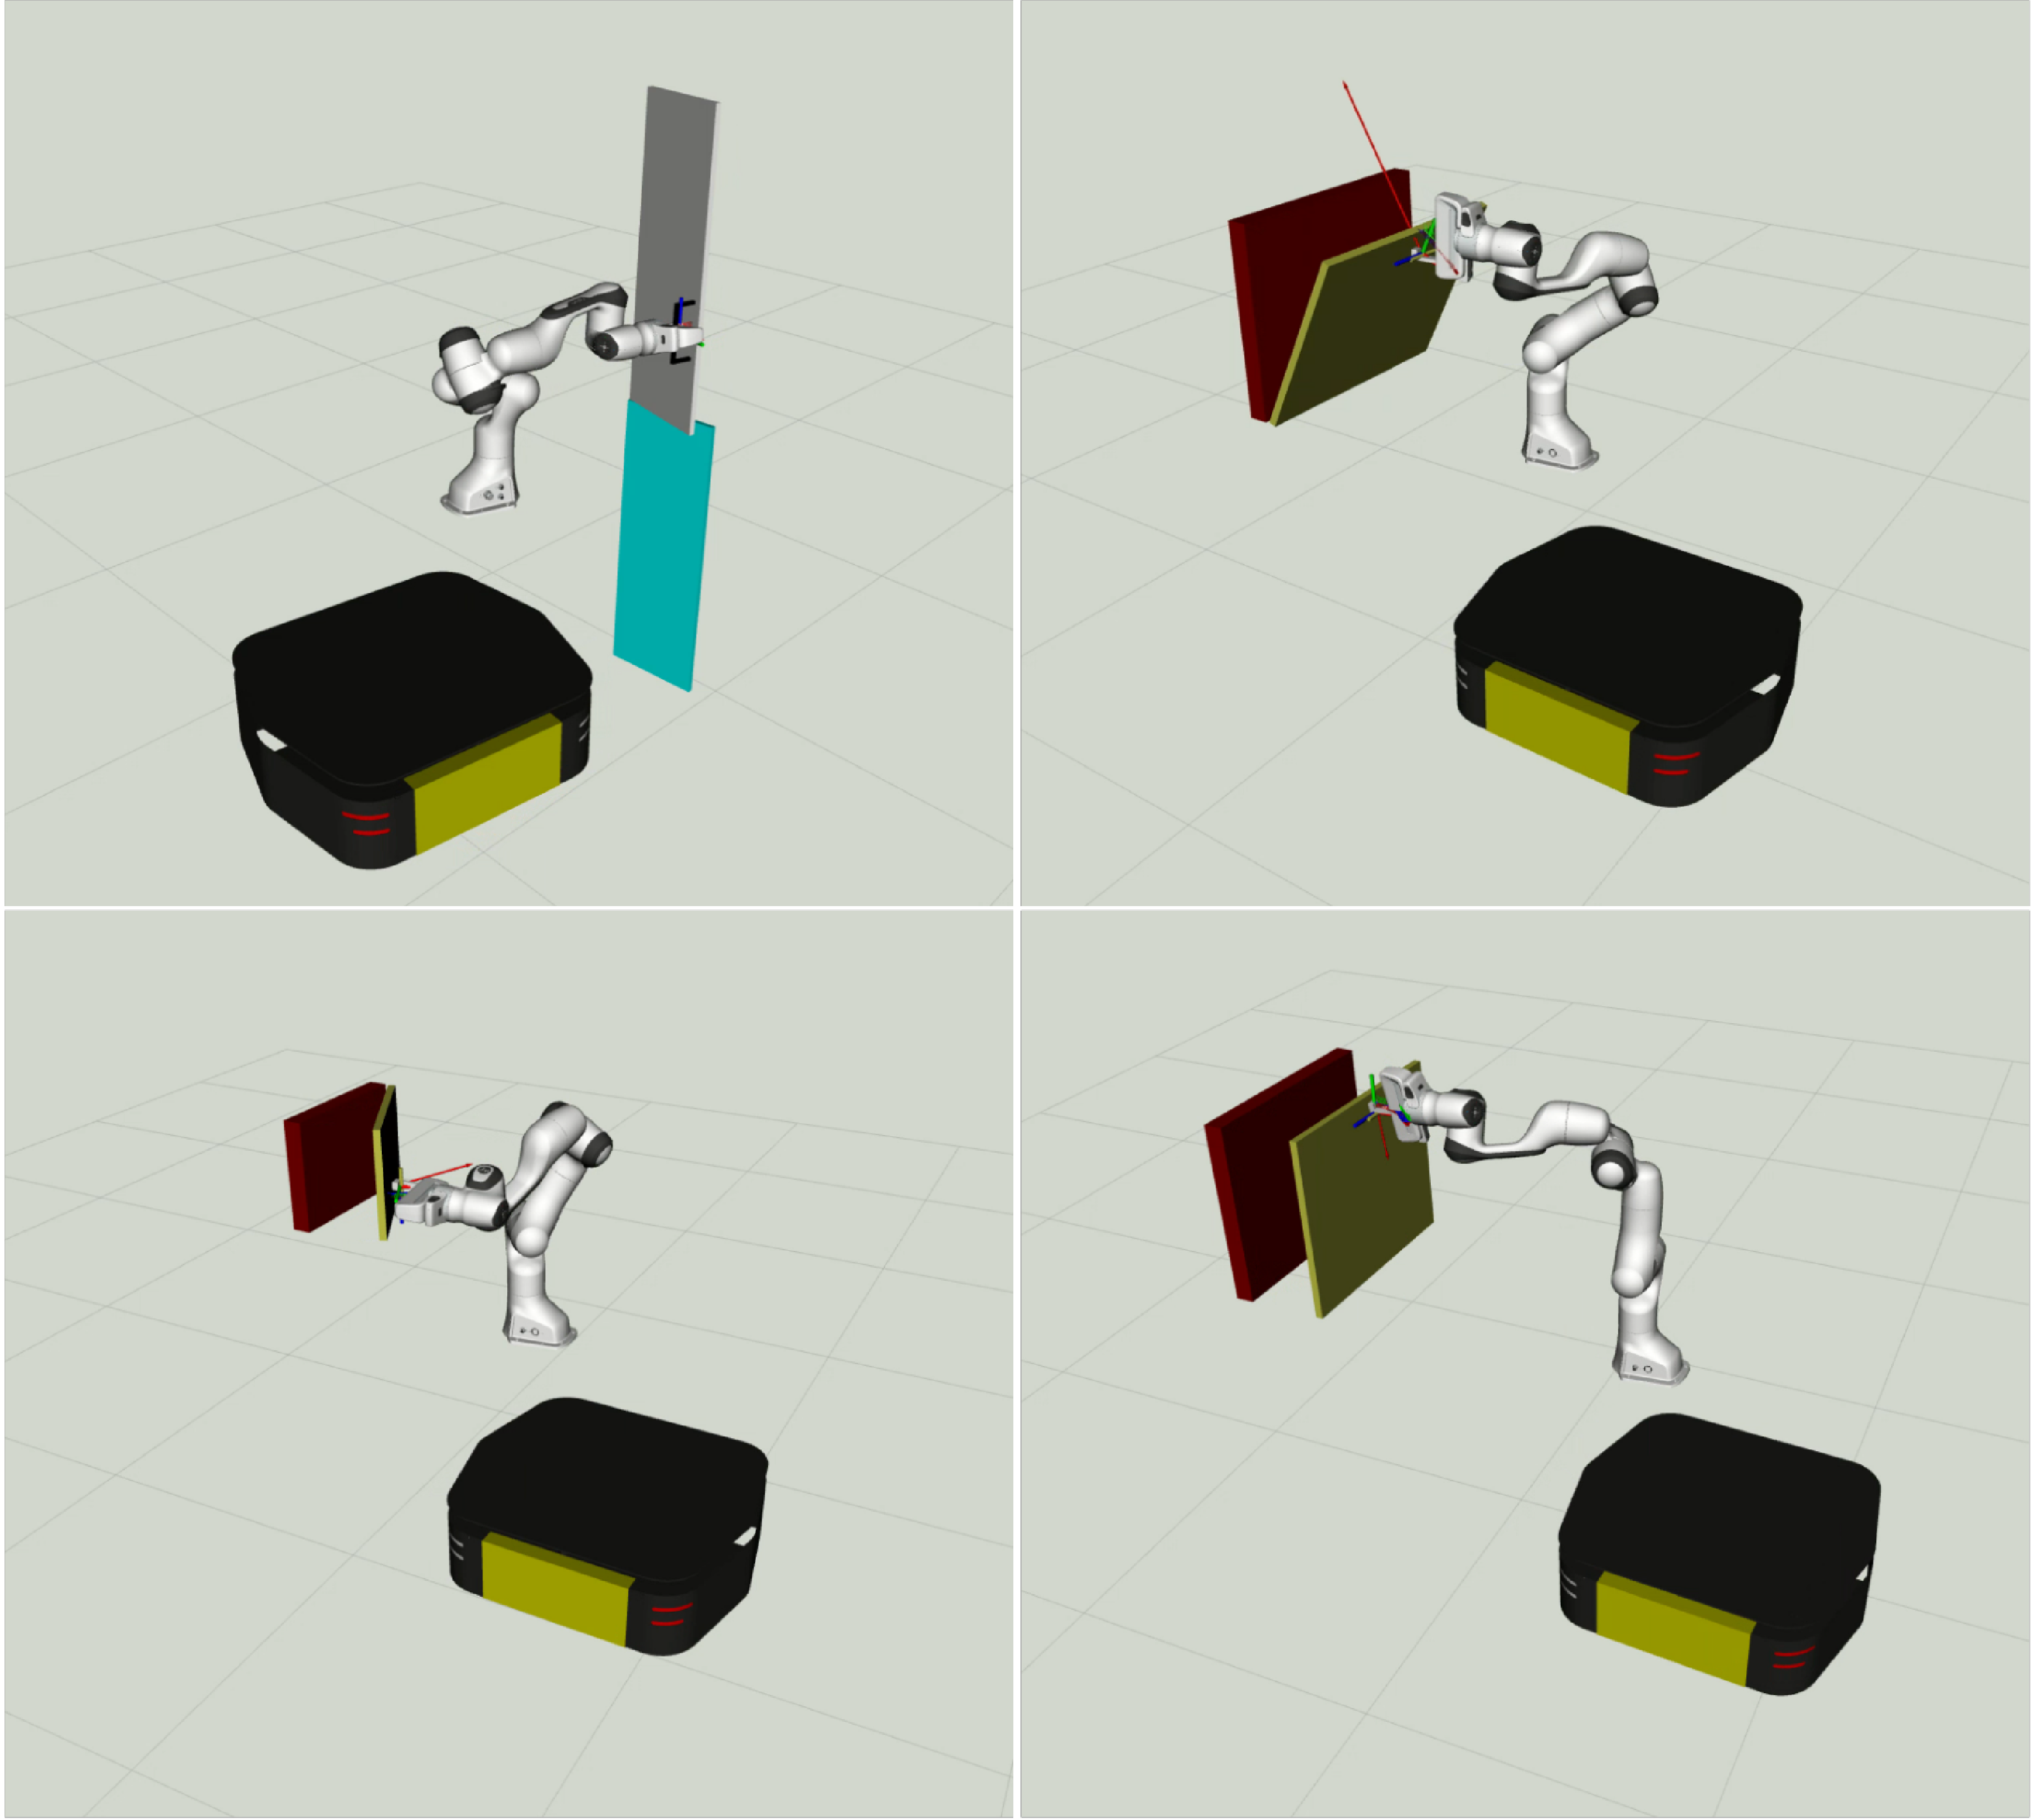
\includegraphics[width=0.7\columnwidth]{framework_manipulation/figures/mosaics/articulated_objects_sim_2x2.pdf}
  \caption{The four articulated objects used in our simulation evaluations. From left to right: \textit{shelf}, \textit{dishwasher}, \textit{microwave} and \textit{drawer}.} \label{fig:object_manipulation}
\end{figure}


The control methods are deployed on the RoyalPanda mobile manipulator and evaluated through simulated and hardware experiments. The platform consists of an holonomic mobile base equipped with a 7-DOF manipulator. The robot's wrist mounts a 6 axis force-torque sensor and a custom set of fingers as shown in \fig\ref{fig:hook_finger}.  The omnidirectional base is controlled by sending velocity commands to the mecanum wheel controller. The arm's low-level controller runs at 1KHz while the base mecanum controller runs at 50Hz. \sout{In order to reduce the sim-to-real gap, in all the simulated experiments, imperfect velocity control is modeled by compensating only 90\% of the gravity terms. }In both the real and simulated robot, the arm velocity commands are converted to joint torques using a PI low-level velocity controller running at 1KHz. 

%\subsection{Power consumption}
%In this experiment we look at the effect of the power term in the task execution. As we can see in \fig \ref{fig:power_cost_comparison}, the power cost is effective in decreasing the energy dissipation during the manipulation task. For each of the experiments where the power cost is active we set $w_p=10$ and $p_{max} = 0.0$. For all experiments we use $50$ samples as they are a good trade-off between control-frequency and performance. We observe that in all experiments the robot is able to accomplish the task (fully open the articulated object). 

%\begin{figure}[t]
%\centering
%  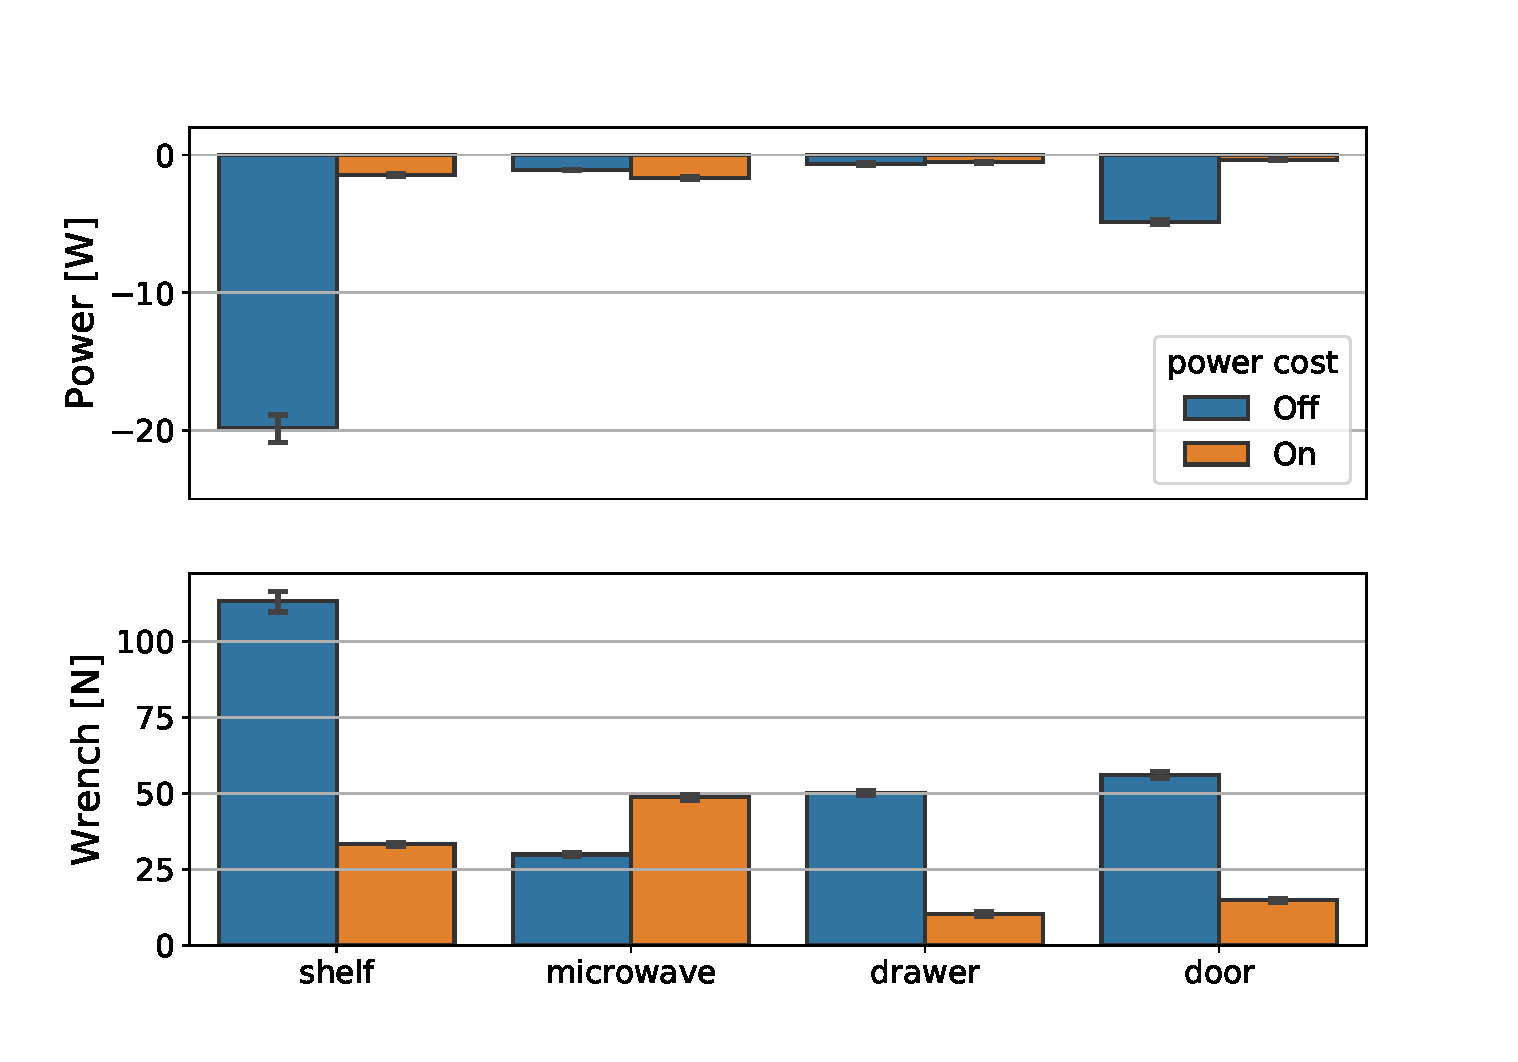
\includegraphics[width=\columnwidth]{figures/methods_comparison/power_cost.pdf}
%  \caption{Power dissipated and wrench norm for each of the manipulated objects.} \label{fig:power_cost_comparison}
%\end{figure}


\subsection{Comparison of Methods}
We design the following experimental scenarios:
\begin{enumerate}
    \item \textit{Object manipulation}: we validate the applicability of the method on the task of manipulating each of the four articulated objects. \add{In each environment there is an handle that the robot can use to move the articulated object. In a first step the end effector reaches the handle and then tries to make contact and move the articulation to the desired position. The switch between hand reaching and object manipulation is triggered turning on the object reference cost as described in \sect\ref{sec:control_method}}. 
    \item \textit{Target reaching and obstacle avoidance}: we further investigate the validity of the constraints formulation for a target reaching task in a confined environment. \add{The end effector must reach a target goal while the base is constrained in a narrow corridor. Furthermore, the robot must avoid an obstacle represented as red sphere in \ref{fig:obstacle_avoidance}. The obstacle is not immediately visible but appears all of a sudden, challenging the reactive response of the sampling-based controller.} \sout{when an obstacle is suddenly placed in the workspace.}
    \item \textit{Robust interaction}: we construct a challenging manipulation scenario where robust interaction is needed; in this case, the articulated object is fixed rigidly and is not able to move for a short period of time.
    \item \textit{Real-world experiments}: we further test the methods on the real robot for a door opening task. 
\end{enumerate}

We run the presented algorithms on a Intel Core i7-8550U quad-core processor (1.8 GHz, up to 4.0 GHz) and use 8 threads for parallel forward sampling of rollouts. Forward simulation is provided by the \texttt{raisim} physics engine \cite{raisim}. The FILTER-QP and Sequential FILTER-QP are solved efficiently using the \texttt{osqp} C++ library \cite{osqp}. We measure an average solving time of $\approx 0.1$ ms. Finally, the main control parameters are summarized in \tab \ref{tab:parameters}.  


\vspace{0.3cm}
\subsubsection{Object manipulation}
We would like to investigate the performance of the algorithms when working close or outside the safety boundaries. To this end, in all the simulated experiments the robot starts in a configuration that is near the arm's joint limits and self-collision. The base of the robot is at $(-3.0, -3.0)$, outside of the prescribed position limits of $[(2.0, 2.0), (-2.0, -2.0)]$. The task of the robot is to open an articulated object moving from its starting location. We perform 20 runs for each articulated object and for each control method.

The results of the experiments are summarized in \fig \ref{fig:methods_comparison}. We observe a reduction of cumulative joint limit violations as well as self-collision violations. We deduce that filtering the input sequence has a beneficial effect. $\Pi_{I}$ and $\Pi_{IO}$ attain the best performance suggesting that in a low sampling regime, the optimization problem helps to adapt the input sequence to quickly reduce the amount of constraint violation. The third row of \fig \ref{fig:methods_comparison} also shows that the naive controller $\Pi_{N}$ even experiences a dramatic failure which is not visible because of plot limits. This edge case never happens for the other methods. 

The dissipated power is similar across the proposed methods although filtering seems to also have a positive effect in this aspect. A qualitative analysis has shown that the interaction wrench measured during a simulated rollout can be inaccurate, especially when the rollouts use big time steps (0.015 s) in order to trade-off simulation accuracy with speed. As the wrench information is used to evaluate the system passivity, we activate the passivity enforcing constraint only in the outer-loop FILTER-QP since this optimization problem consumes real wrench measurements at high rates. This choice is additionally justified by the fact that passivity is mainly a mechanism designed to react to unforeseen events. As these are not modeled, the simulated rollouts are not able to predict the true evolution of the interaction wrench and therefore when passivity is enforced throughout the rollouts it could lead to detrimental effects, namely an implementation of a non-passive behavior on the real robot.


Overall, the simulated experiments confirm the validity of the full framework (as implemented in $\Pi_{IO}$). Nevertheless the performance differences are not striking. We think that this is due to the low chance of hitting the constraints during the task, especially when the sampling-based controller is aware of dangerous configurations through a well-engineered cost function. In fact, high cost on safety-related objectives has the effect of ``trimming" bad trajectories, removing the need for the post-processing performed by the constrained optimization problem. For this reason, in the following we present a second simulation experiment which represents a challenge for a purely sampling-based controller. 

\begin{figure}[t]
\centering
\hspace*{-0.2cm}
\vspace*{0.15cm}
\begin{subfigure}{1\columnwidth}
    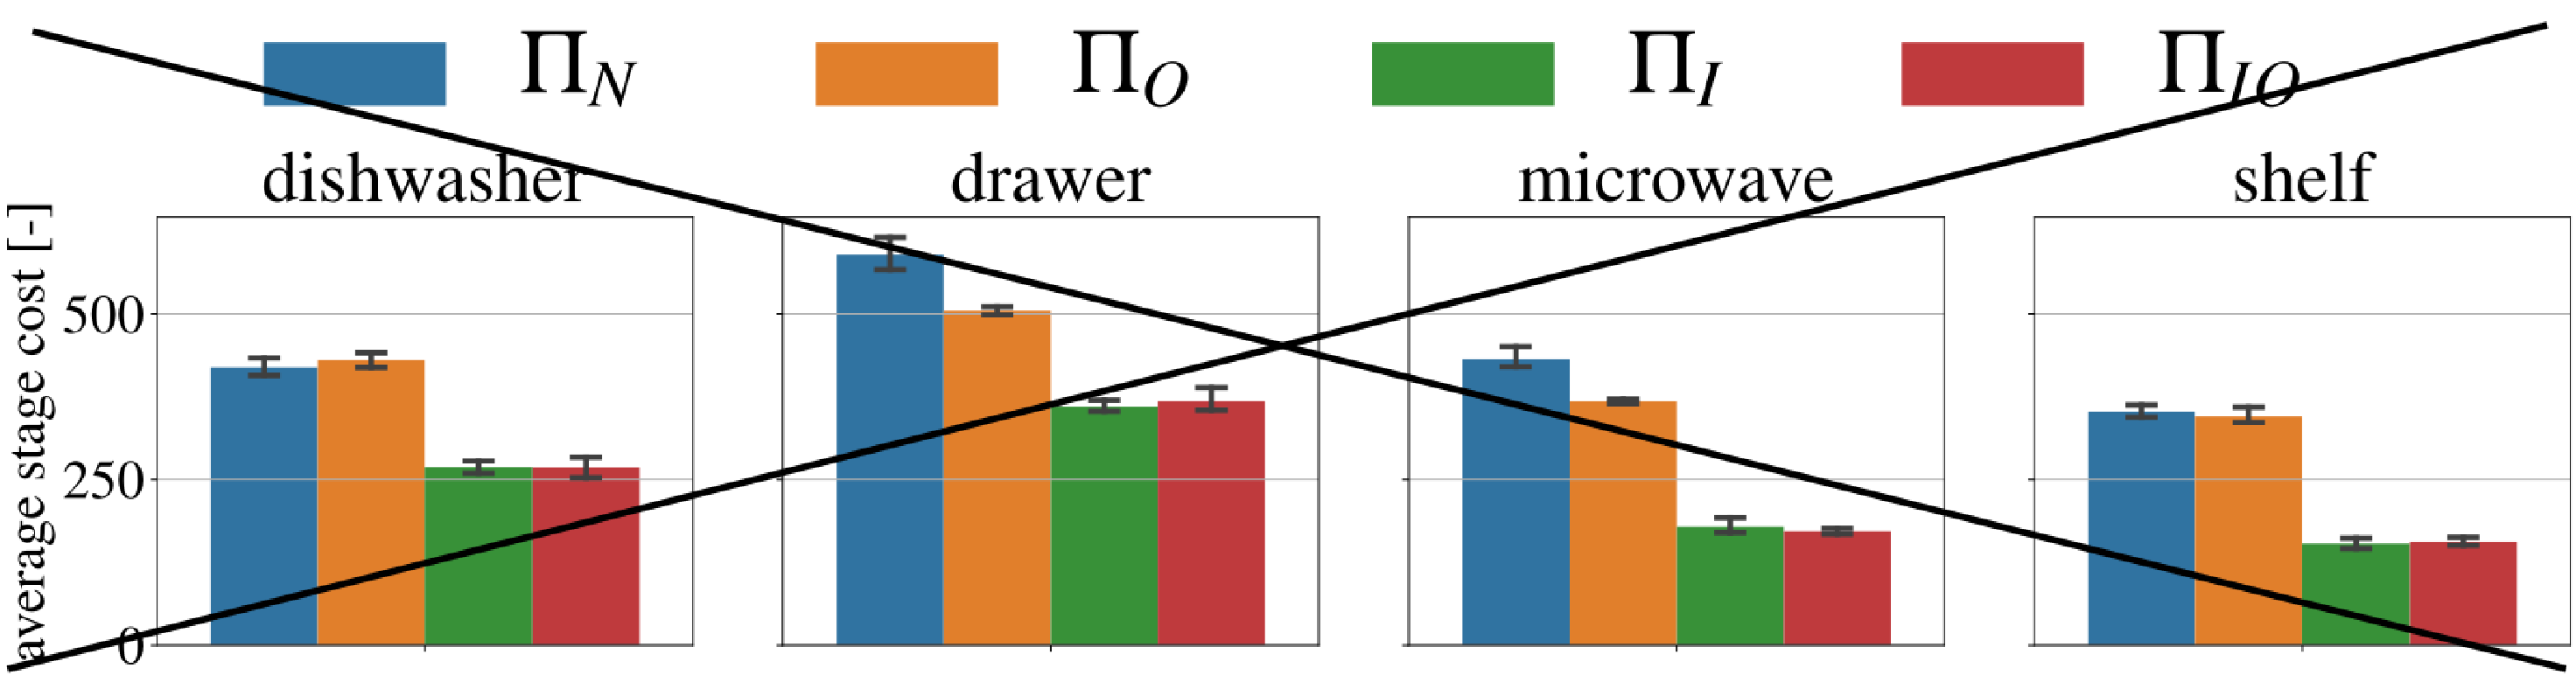
\includegraphics[width=\linewidth]{figures/methods_comparison/average_stage_cost_sout.pdf}
\end{subfigure}%
\hfill
\begin{subfigure}{1\columnwidth}
    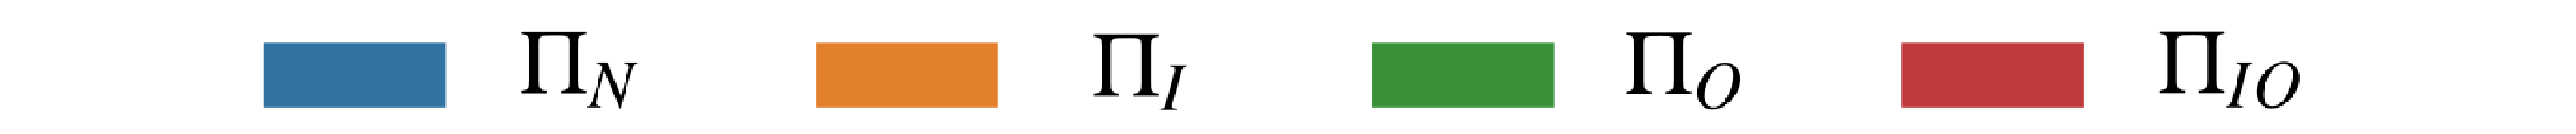
\includegraphics[width=\linewidth]{figures/methods_comparison/legend.pdf}
\end{subfigure}%
\hfill
\hspace*{-0.2cm}
\vspace*{0.1cm}
\begin{subfigure}{\columnwidth}
    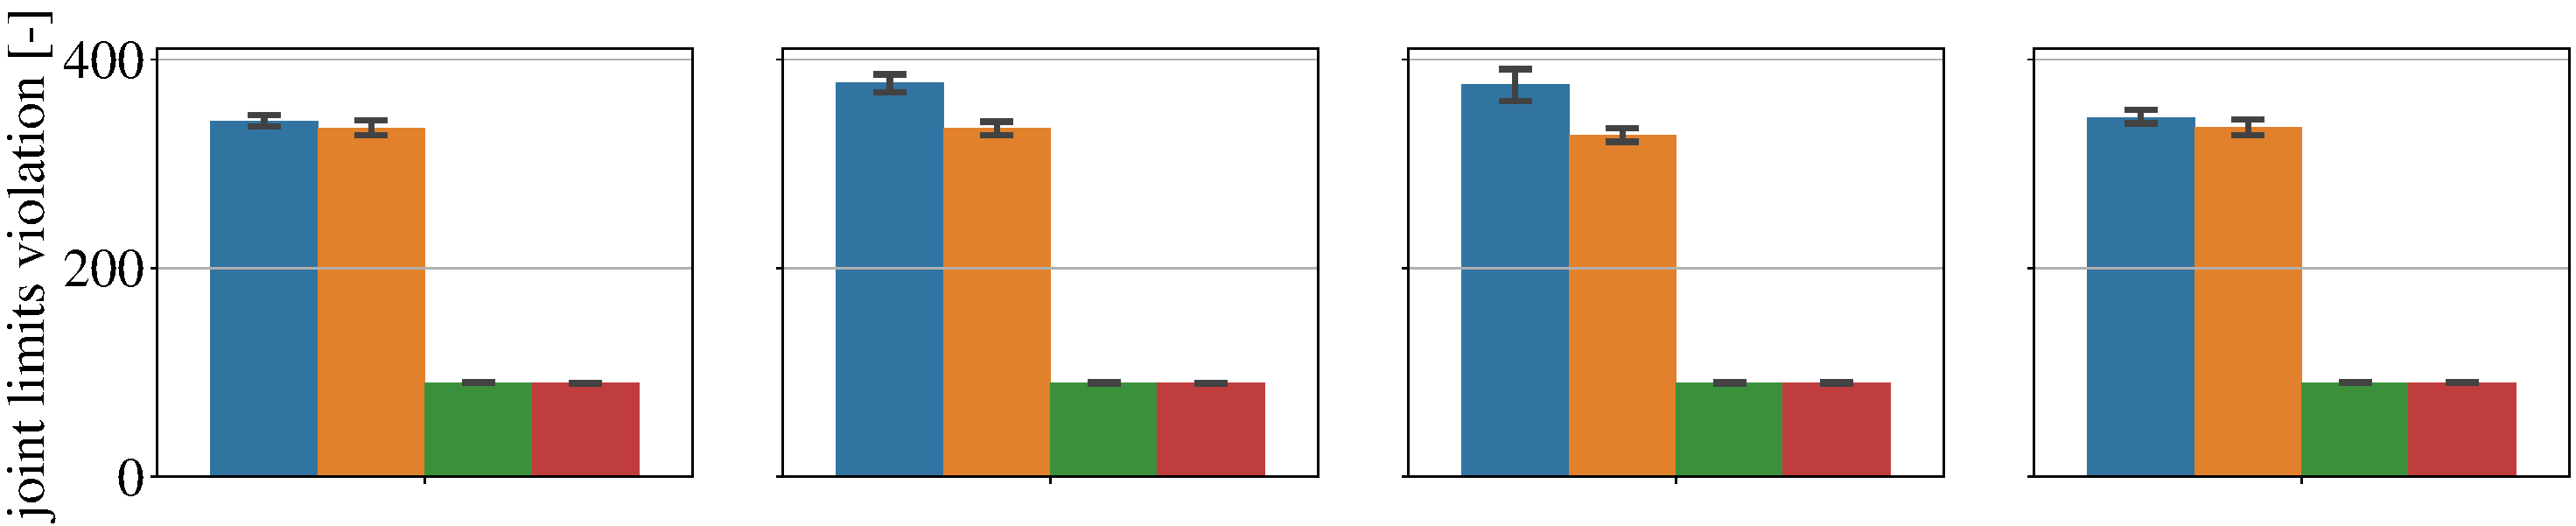
\includegraphics[width=\linewidth]{figures/methods_comparison/joint_limits.pdf}
\end{subfigure}%
\hfill
\hspace*{-0.2cm}
\vspace*{0.1cm}
\begin{subfigure}{\columnwidth}
    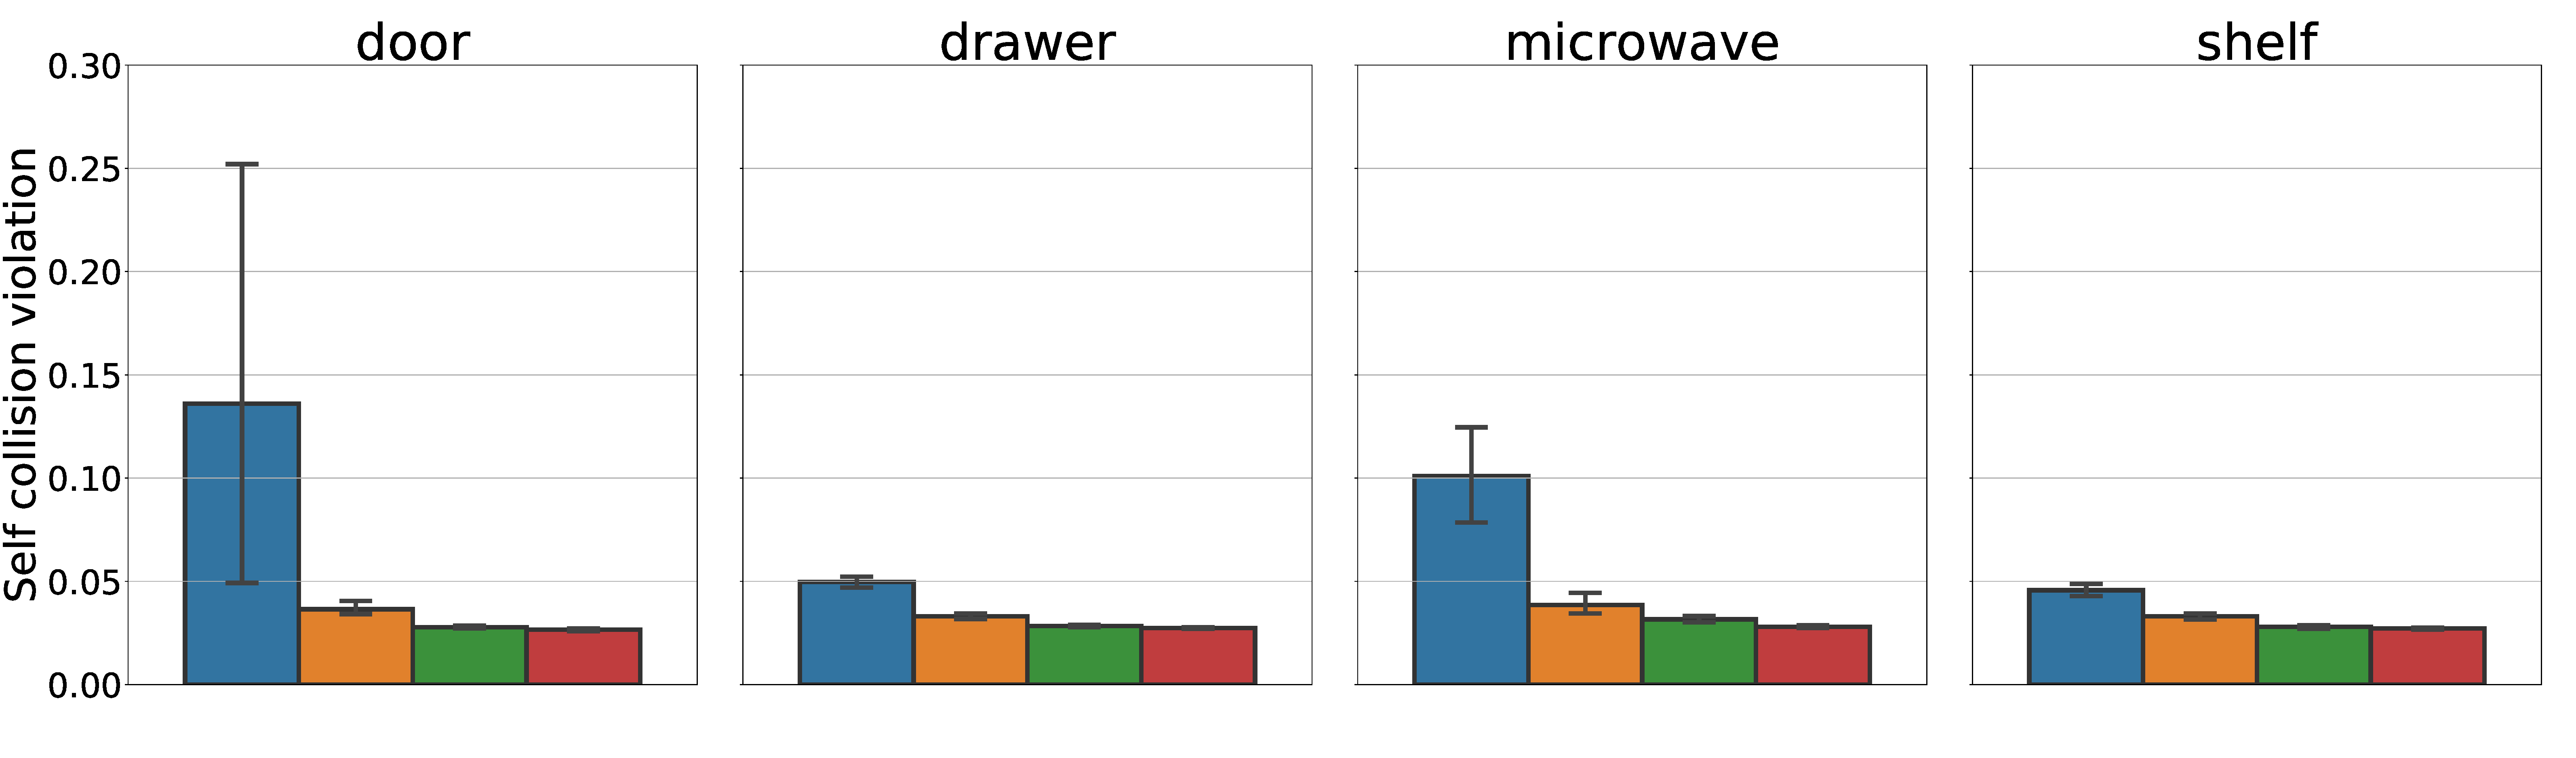
\includegraphics[width=\linewidth]{figures/methods_comparison/self_collision.pdf}
\end{subfigure} %\label{fig:self_collision_violation}
\hspace*{-0.2cm} 
\vspace*{0.1cm}
\begin{subfigure}{\columnwidth}
    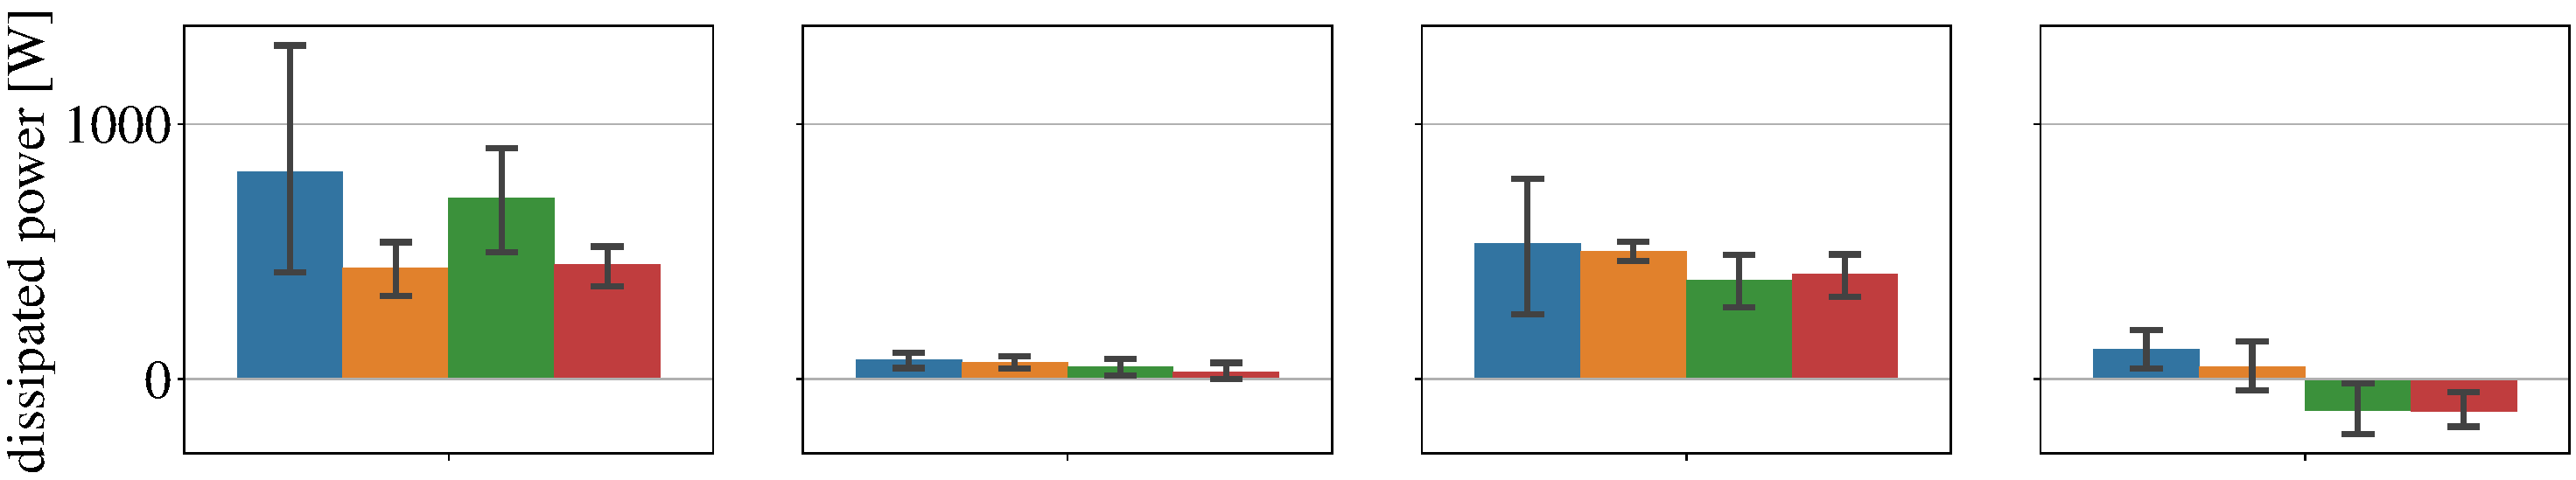
\includegraphics[width=\linewidth]{figures/methods_comparison/dissipated_power.pdf}
\end{subfigure}
\hfill
\caption{Comparison between the different control methods. Note that The self-collision barplot has a data point at $3.4$ in the $\Pi_{N}$ method for the \textit{dishwasher} case, which is far outside the plot range.}\label{fig:methods_comparison}
\end{figure}

\vspace{0.3cm}
\subsubsection{Target reaching and obstacle avoidance}
The naive stochastic controller relies on a task-encoding cost formulation and sampling to generate ``good" rollouts. This method faces two main challenges:
\begin{itemize}
    \item the cost needs to be nicely tuned in order to prevent edge cases where performance is chosen in lieu of safety,
    \item sudden changes in the cost function lead to a drastic change in the policy distribution.
\end{itemize}
While the first issue can be addressed by tuning the cost with a trial-and-error method, the second is more subtle. In fact, the policy should be able to quickly adapt but this can be hard to achieve when only sampling around the previous (outdated) input distribution. In this experiment we reproduce the described issue during a target reaching task. We place a collision sphere at each robot link and an obstacle in the robot workspace. The base motion is also constrained such that, in order to achieve the goal, the robot is forced to avoid the obstacle while going through a narrow passage. The obstacle is perceived only when the robot is very close to it ($<$ 1cm) causing a sudden change in the cost function. We show the end-effector optimal trajectory for $\Pi_{N}$ and $\Pi_{IO}$ after the obstacle has been detected in \fig \ref{fig:rollouts_comparison}. We can see that the naive controller $\Pi_{N}$ is not able to quickly adapt to the unforeseen cost change and instead is trapped in a high cost region where it is hard to find a good trade-off between obstacle avoidance and the target reaching objective. In contrast, the $\Pi_{IO}$ controller immediately adapts the input sequence to comply with the constraints and sampling can later be performed in a more favorable region of the input space.   

\begin{figure}[t]
\centering
\begin{subfigure}{0.48\columnwidth}
    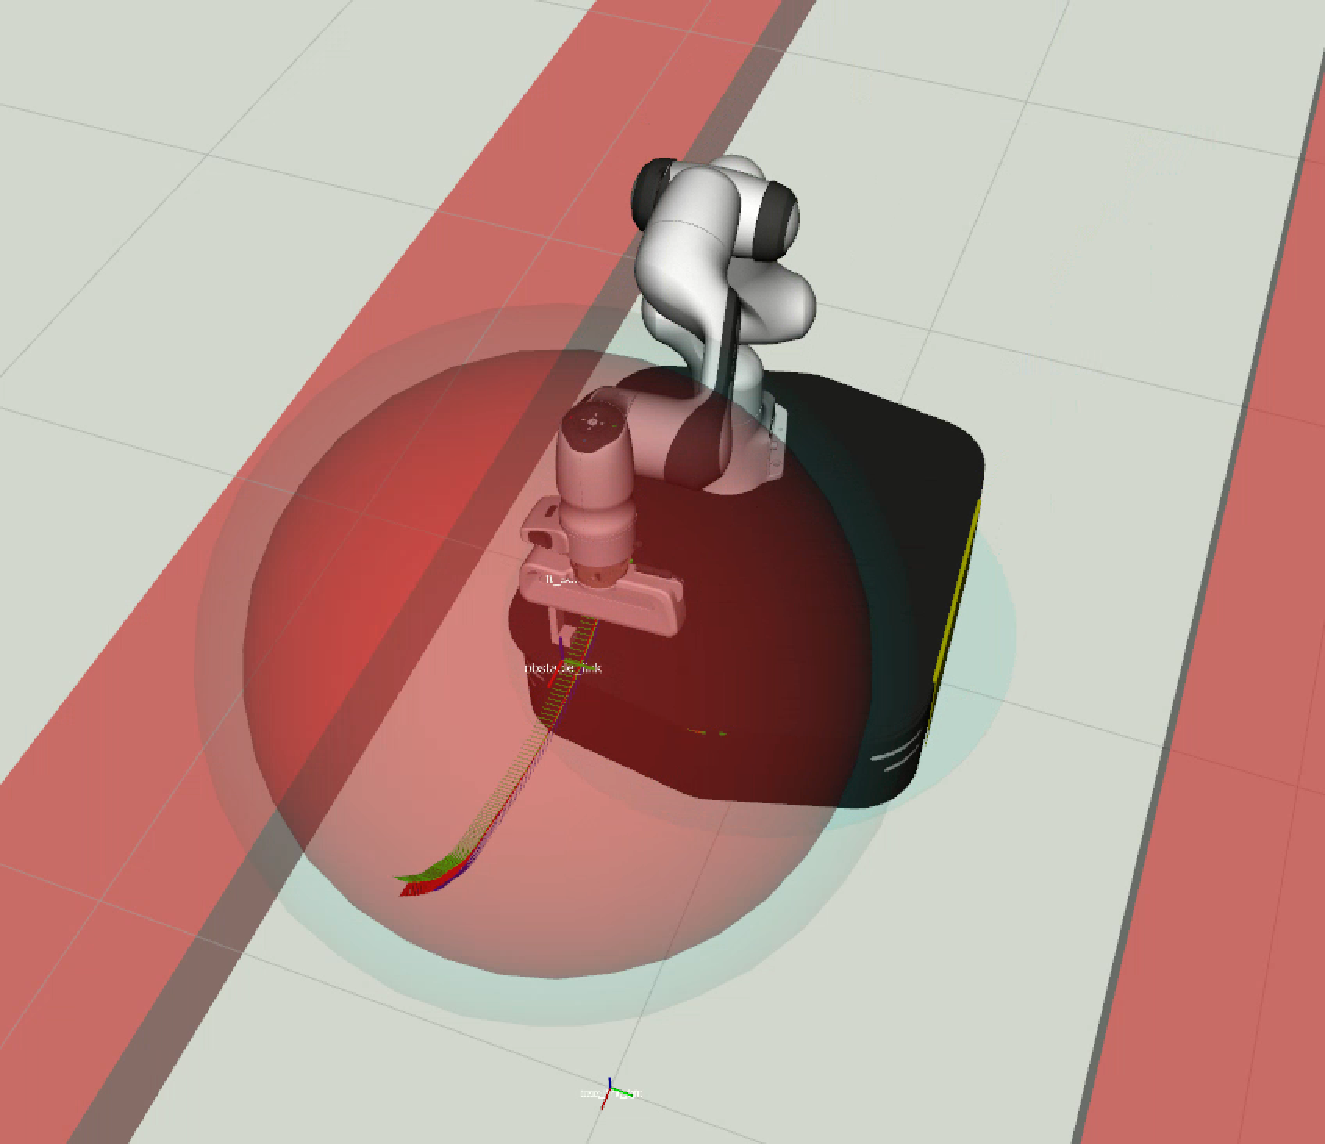
\includegraphics[width=\linewidth]{figures/obstacle_avoidance/rollouts_no_filter.pdf}
    \caption{Example rollout of $\Pi_{N}$}
\end{subfigure}%
\hfill
\begin{subfigure}{0.48\columnwidth}
    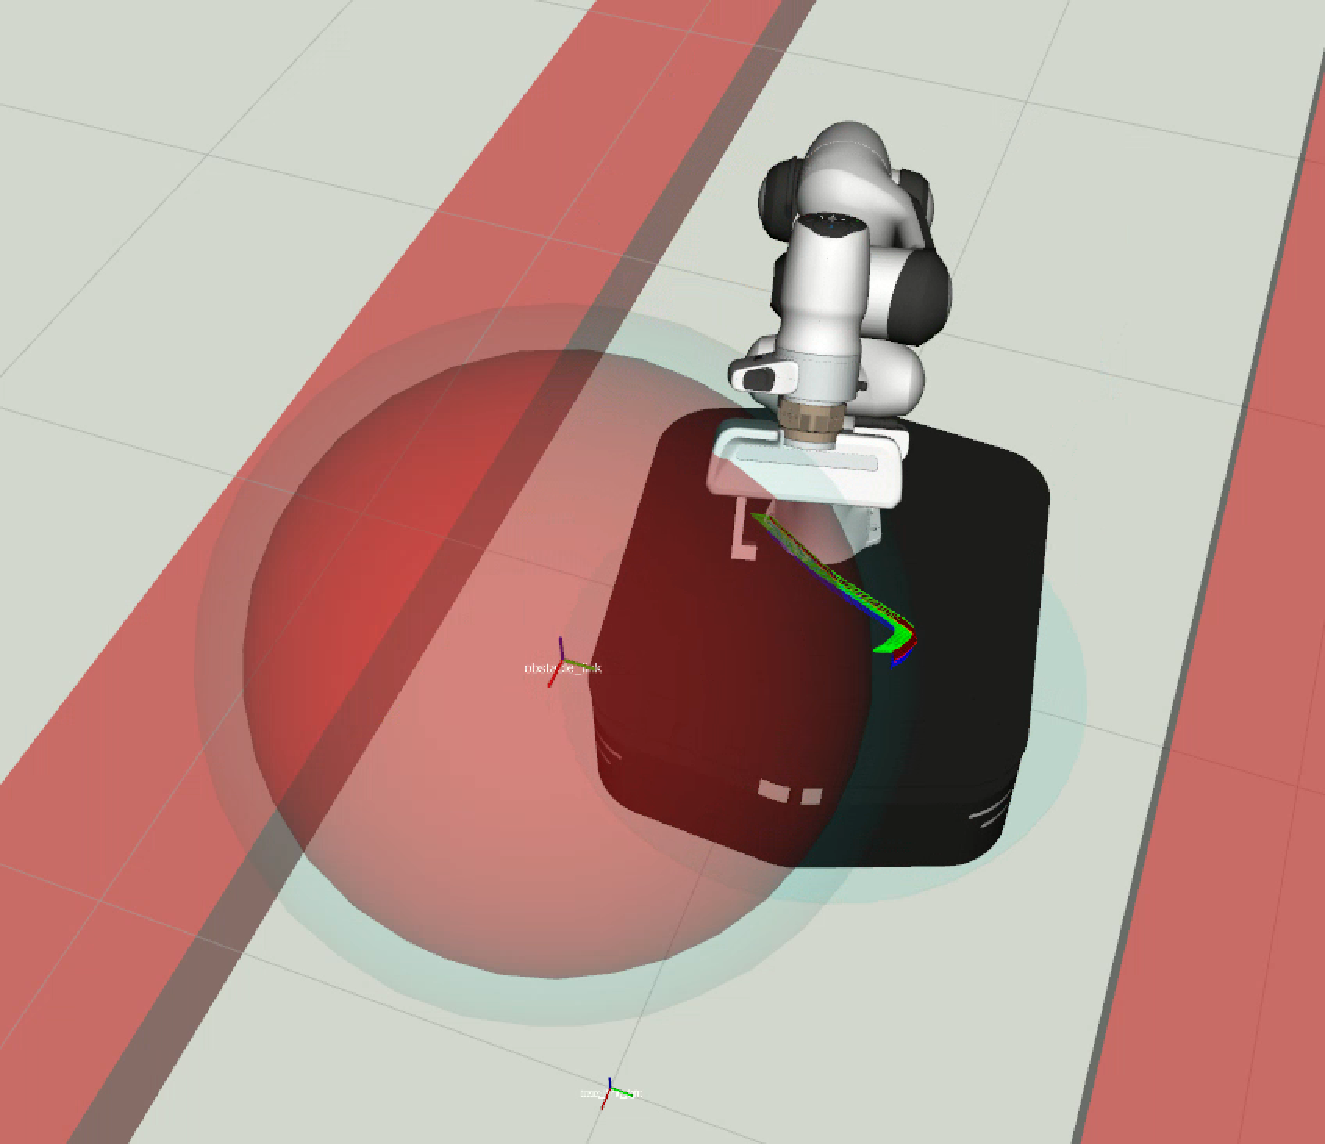
\includegraphics[width=\linewidth]{figures/obstacle_avoidance/rollouts_filter.pdf}
    \caption{Example rollout of $\Pi_{IO}$}
\end{subfigure}%
\hfill
\caption{In the figure we visualize the optimized end-effector trajectory by rolling out the optimized command. The naive controller $\Pi_{N}$ is trapped in a high cost region while $\Pi_{IO}$ immediately reacts to the unexpected cost change.}\label{fig:rollouts_comparison}
\end{figure}

We repeat the simulation for 10 runs for each of the methods. The results are summarized in \fig \ref{fig:obstacle_avoidance}. As expected, $\Pi_{IO}$ attains the best performance. We further observe that the presence of a FILTER-QP in the outer high-rate loop additionally improves robustness as it enforces constraints during the open-loop execution of the optimized trajectory received by the stochastic controller. 
\begin{figure}[t]
\begin{subfigure}{1\columnwidth}
    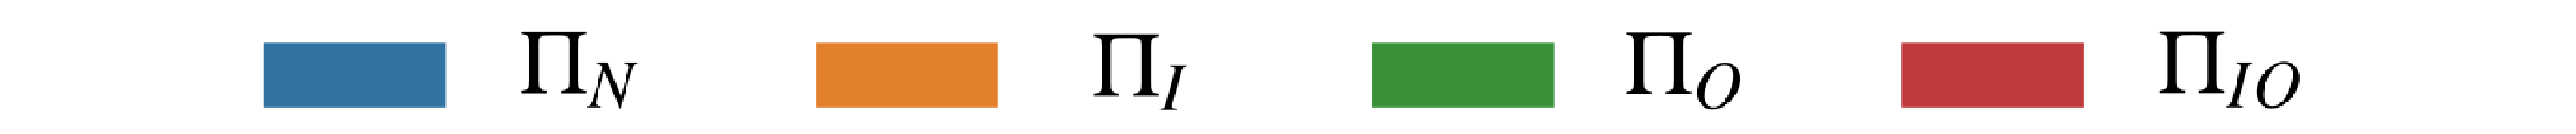
\includegraphics[width=\linewidth]{figures/methods_comparison/legend.pdf}
\end{subfigure}%
\hfill

\begin{subfigure}{1\columnwidth}
    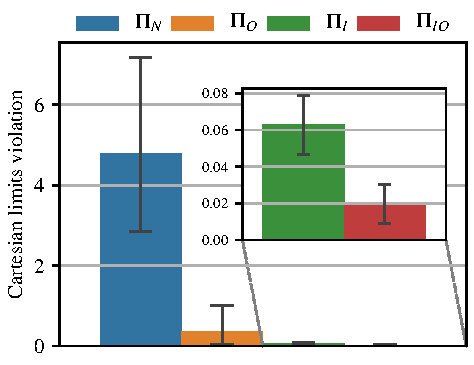
\includegraphics[width=0.7\columnwidth]{figures/obstacle_avoidance/obstacle_avoidance_test.pdf}
    \caption{The barplot shows the cumulative cartesian limits violation for the target reaching and obstacle avoidance task. $\Pi_{I}$ already outperforms $\Pi_{N}$ and $\Pi_{O}$. A further small performance boost is achieved by $\Pi_{IO}$.}
    \label{fig:obstacle_avoidance}
\end{subfigure}
\end{figure}

\vspace{0.3cm}
\subsubsection{Robust interaction}
The previous validations show how the framework can address manipulation tasks and overcome some limitations of a naive stochastic controller. We aim to find evidence that the additional passivity enforcing constraint adds robustness to the method. By adding the energy tank constraint to the optimization problem, we limit the maximum dissipated energy and thus generate a stable interaction behavior.

To evaluate this, we alter the \emph{shelf} scenario described earlier such that the motion of the shelf door is limited while the robot is interacting with it. We fix the door position for $5$ seconds, simulating it becoming ``stuck". After this time, the object is released and is free to move within its original limits again. This experiment could approximate a real scenario where the object is temporarily constrained because of defects in the opening mechanism or joints' wear.

From the results in \fig \ref{fig:tank_comparison}, we note that when using $\Pi_{N}$, i.e., no passivity is ensured, the negative power flow is not bounded, leading to high interaction wrenches. On the other hand, when the energy tank is deployed, as in $\Pi_{IO}$, only a maximal amount of energy, namely that stored in the tank, can be used. Furthermore, we use a small value of $\alpha=1$ in the passivity constraint formulation \eqref{eq:passivity_simple}. As discussed in \sect \ref{sec:practical_aspects} and shown in \fig \ref{fig:tank_as_zbf}, this choice allows for a smoother power regulation when approaching the lower energy bound when compared to larger values of $\alpha$ and prevents chattering. 

\begin{figure}[t]
\centering
\begin{subfigure}{\columnwidth}
\centering
    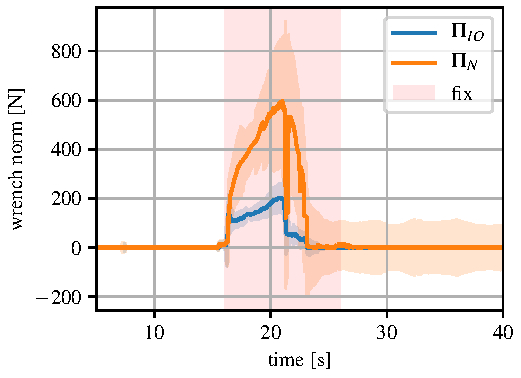
\includegraphics[width=0.8\linewidth]{figures/fix_experiment/wrench_with_without_tank.pdf}
    \caption{The  \textcolor{orange}{\textbf{orange}} shaded area shows the time interval when the object is fixed. Note that this might vary for each experiment as the object reaches the prescribed position at different time points.}
\end{subfigure}
\begin{subfigure}{\columnwidth}
\centering
    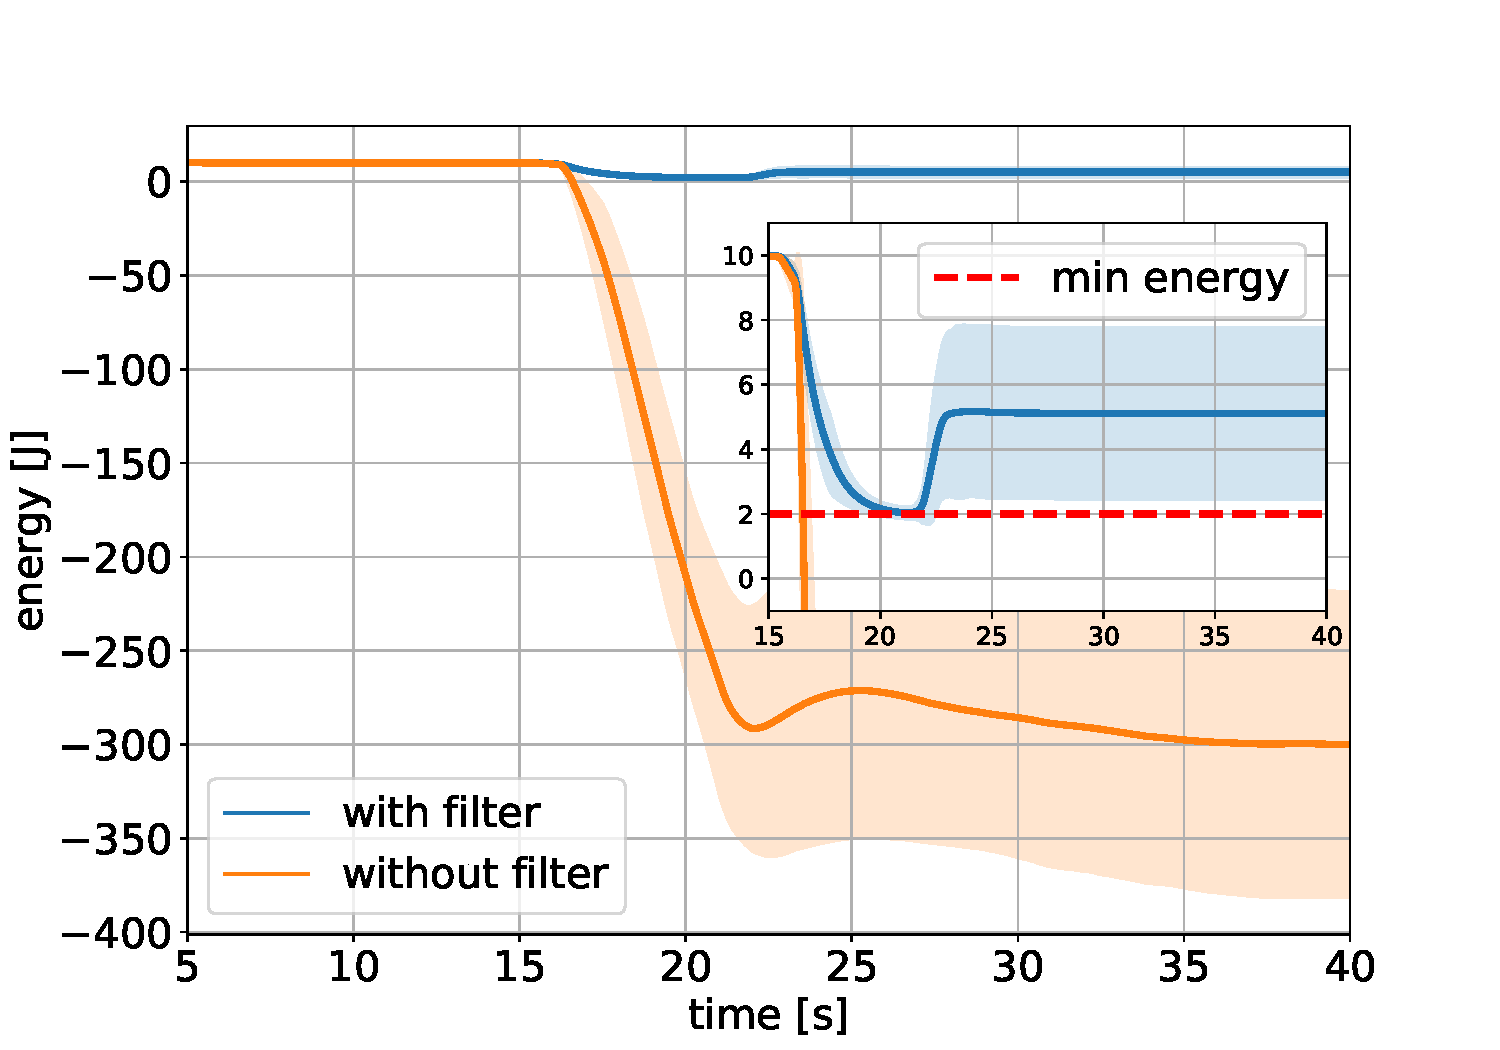
\includegraphics[width=0.8\linewidth]{figures/fix_experiment/energy_with_without_tank.pdf}
    \caption{The energy of the tank when the filter is deployed (\textcolor{red}{\textbf{red}} curve) is always above the prescribed minimum, while it drastically drops in the other case. The plotted energy is computed integrating the dissipated power during interaction.}
\end{subfigure}
\hfill
\caption{The filter regulates the dissipated power when energy is low in the tank, resulting in a reduced wrench when the object is ``stuck". The line plot and shaded area show the mean and standard deviation from 20 simulation runs of interaction with the \textit{shelf} object respectively.}\label{fig:tank_comparison}
\end{figure}

\begin{figure}[t]
\centering
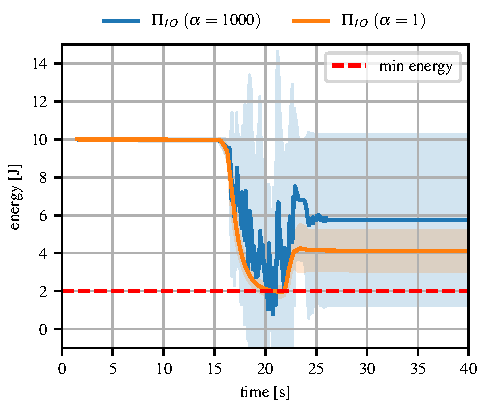
\includegraphics[width=0.8\columnwidth]{figures/fix_experiment/passivity_coefficient_comparison.pdf}
\caption{In this figure we show the chattering effect happening when the constraints are enforced with $\alpha = 1/dt = 1000$. In contrast, a lower $\alpha$ greatly alleviates this issue.}\label{fig:tank_as_zbf}
\end{figure}

\vspace{0.3cm}
\subsubsection{Real-world experiments}
The goal of the hardware experiments is to demonstrate that the algorithm can be deployed on a real platform in a real-time setup. For this purpose, we perform a door opening experiment similar to the description provided in the previous section with our RoyalPanda robot. The door displacement and the robot's base are tracked using a motion tracking system, eliminating the need for precise state estimation. We plan to remove this limitation in future work. The door motion is limited using a rope. We monitor the evolution of the tank energy and once it has reached the allowed minimum we wait 3 seconds before manually cutting the rope. We repeat the experiment for the methods $\Pi_{N}$ and $\Pi_{IO}$ recalling that the latter only uses the passivity constraint in the outer loop.

The wrench norm and the evolution of the energy in the tank during the experiments can be seen in \fig \ref{fig:passivity_experiment}. As one can see in the accompanying video, without passivity, the manipulator exerts a rapidly increasing wrench until the rope is broken apart. On the other hand, when passivity is enforced, the power flow and external wrench is regulated leading to a robust interaction behavior and no need for the operator to intervene. When the object is released, the gripper gets stuck in a constrained configuration between the door plate and the handle. When $\Pi_{N}$ is deployed, the controller tries to push aggressively and is therefore not able to escape this gripper trap. When using $\Pi_{IO}$ instead, the tank residual energy is low and aggressive actions are prohibited. The overall behavior is safer and allows the robot to escape from the bad configuration.  

\begin{figure}[t]
\centering
% \hspace*{-0.0cm} 
\begin{subfigure}{\columnwidth}
\centering
    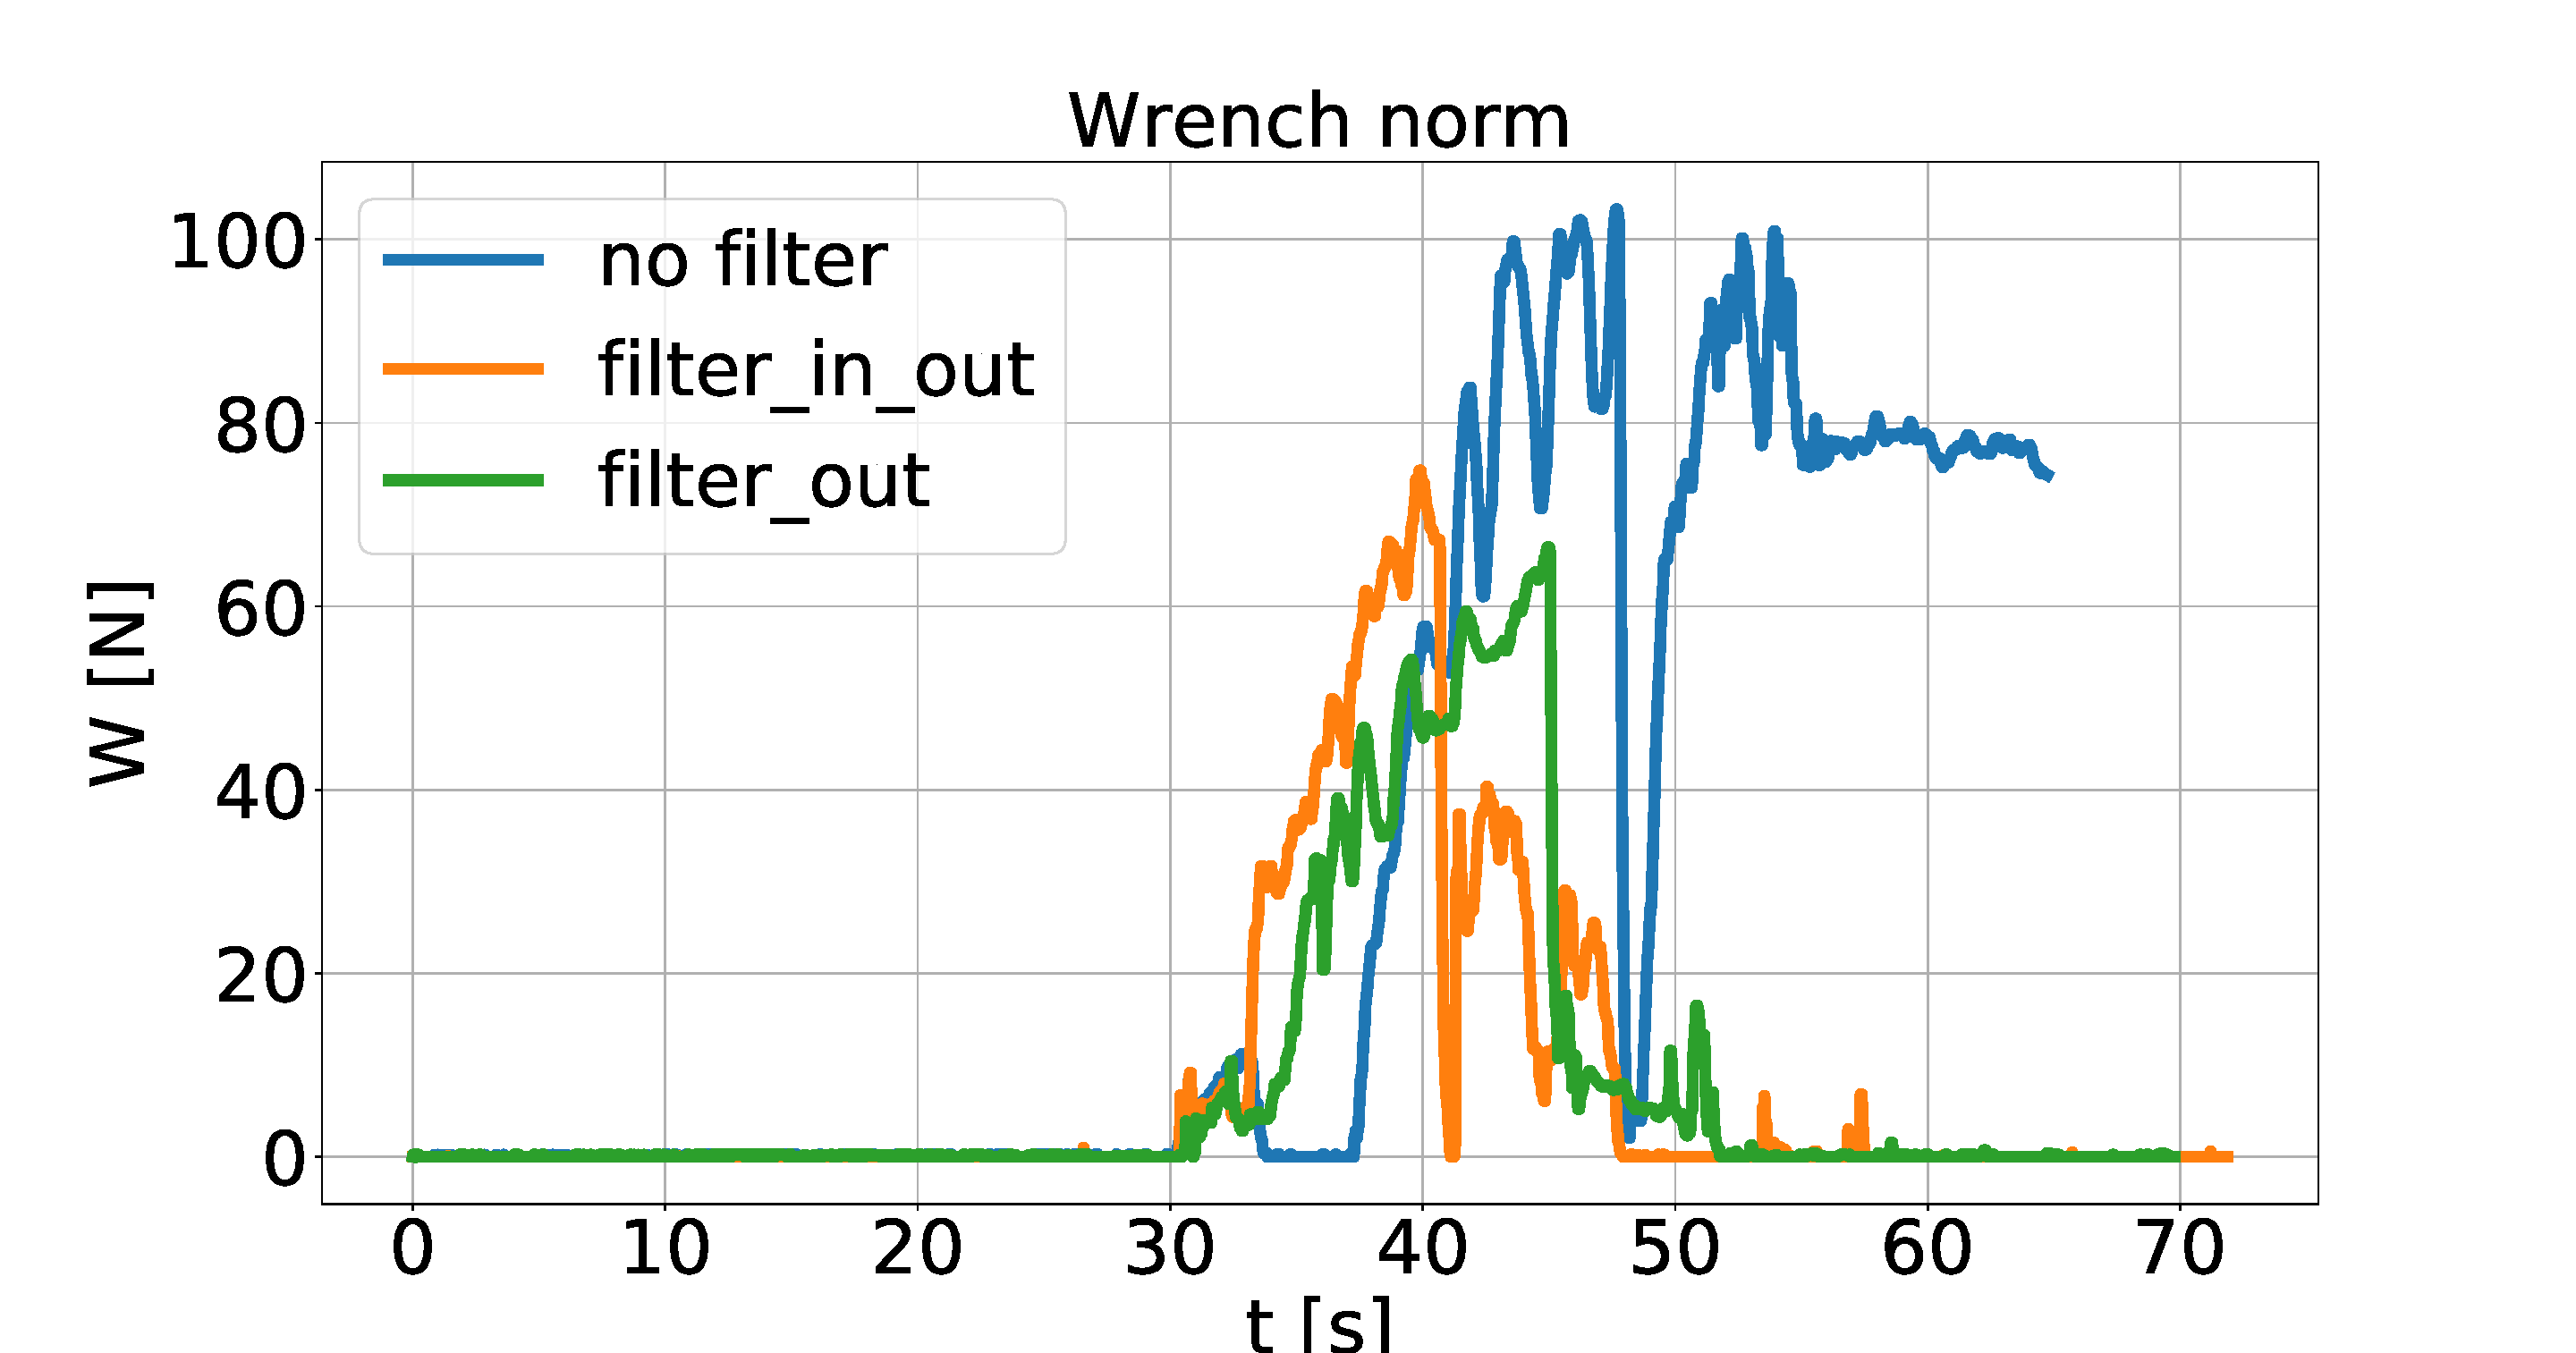
\includegraphics[width=0.7\linewidth]{figures/hardware_experiments/wrench_norm.pdf}
    \caption{Wrench norm during the door opening experiment. We measure an average wrench of 68 N and 34 N for the $\Pi_{N}$ and $\Pi_{IO}$ methods respectively. The sharp wrench drop corresponds to the time when the rope breaks and energy is suddenly released. The two time series have been aligned to facilitate visualization.}
\end{subfigure}
% \hspace*{-0.2cm} 
\begin{subfigure}{\columnwidth}
\centering
    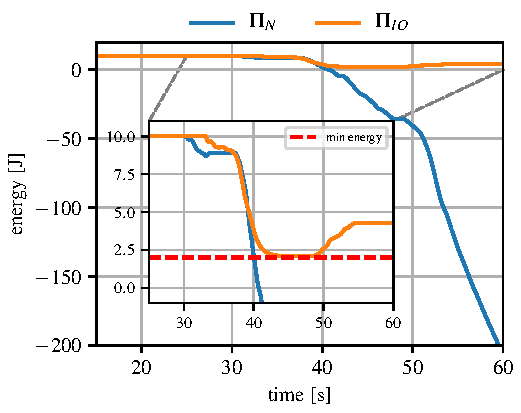
\includegraphics[width=0.7\linewidth]{figures/hardware_experiments/energy_tank.pdf}
    \caption{Evolution of the tank energy over time during the door opening experiment. The zoomed plot shows that energy is recovered when the object is released.}
\end{subfigure}
    \caption{The figures show that when passivity is enforced, the controller is able to limit the overall interaction wrench. This experiment is also reported in the accompanying video.}
    \label{fig:passivity_experiment}
\end{figure}


% In order to qualitatively evaluate the algorithm's replanning capabilities, we disturb the manipulator during the opening phase, releasing the contact between the handle and the finger. As we can see in the accompanying video, the controller is able to re-plan a feasible trajectory to the handle and successfully perform the task. 

\section{Method Limitations and Future Work}\label{sec:limitations_and_future_works}
In the following we describe the most prominent issues that emerged during the experiments and how they could be addressed to improve the proposed method.

\subsection{Model Mismatch}
We have found that the method is highly sensitive to model mismatches. While we can assume that the robot model is known with high accuracy, this is often not the case for the object we intend to manipulate. Unfortunately, we observed that a small uncertainty in the estimate of the object pose and geometry could lead to failures in the door opening experiment. In particular, if the handle placement was not measured exactly, the controller would generate a ``tapping" motion which would cause a hard collision between the finger tip and the handle itself. One can try to quantify the sensitivity of the method to model mismatches and leverage this knowledge to account for the estimate uncertainty. Nevertheless this is not an easy task as there are dependencies across a range of factors, including the specific object geometry, finger design, object placement and articulation type. 

\subsection{State and Model Estimation}
We believe that a tighter integration with perception could be extremely fruitful and help to reduce the amount of prior knowledge needed. A perception system could be devised to extract local 3D patches that are used as candidate interaction hotspots. On the other hand, a surface mesh is not sufficient to model the object motion and dynamical behavior. As a matter of fact, an articulated object is also described by its kinematic parameters, namely the center and axis of rotation. Last but not least, mass, damping and friction could be estimated. However, since we did not tune any of these parameters to accurately match the real articulated object in our experiments, we conclude that the method is less sensitive to uncertainty in these model parameters.

\subsection{Cost Engineering}
The generation of good trajectories strongly depends on a well-engineered and task-dependent cost formulation. With poor cost tuning, stochastic policy optimization, as in the presented method, will tend to become trapped in local minima. Recall that during the manipulation task we rely mainly on two cost components. We use an end-effector pose cost to drive a virtual gripper frame to the location of an interaction frame, located on the medial axis of the handle. This serves as an interaction location prior. A second door-opening cost instead favors trajectories that pull the door open. If the first term is too high relative to the second, sampling could lead to sub-optimal solutions where the end-effector hovers in the proximity of the handle. In fact, pose deviations, from which some are able to successfully pull the door open, are highly penalized.

A second design aspect which influenced sampling quality is the placement of the virtual gripper frame. If this was too close to the finger collision geometry, random sampling would often fail to find a solution that avoids collision and successfully reaches the target pose. Instead, when this is placed at a small offset away from the finger tips one can prevent early collision and successfully reach the prescribed target pose. Both placements are shown in \fig \ref{fig:frame_placement}. While in this work we focus on a practical method for high-rate closed-loop control, a larger sampling budget or a multimodal policy distribution~\cite{lambert_stein_2020} could help to find better solutions but always at the cost of higher compute and lower control rates.

\begin{figure}[t]
\centering
\begin{subfigure}{0.48\columnwidth}
    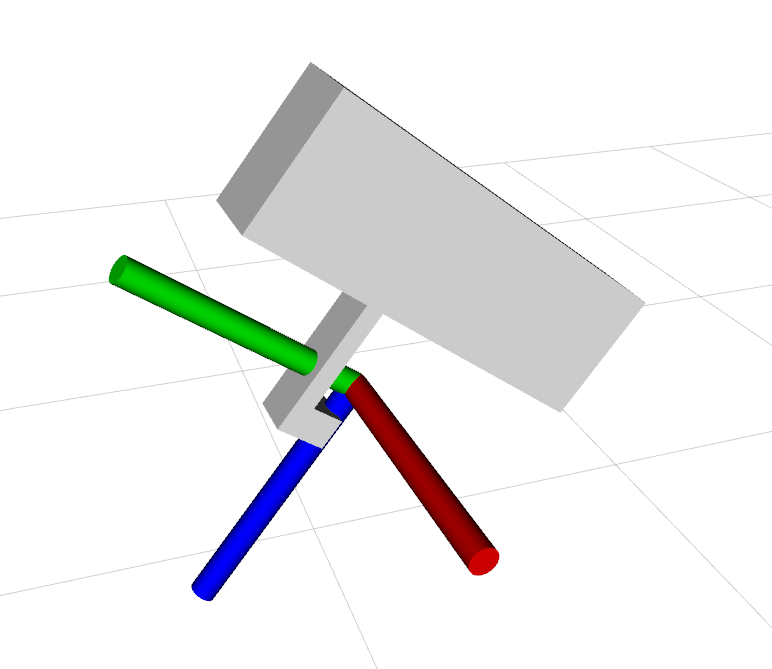
\includegraphics[width=\linewidth]{figures/panda_grasp_2.png}
    \caption{Bad frame placement.}
\end{subfigure}%
\hfill
\begin{subfigure}{0.48\columnwidth}
    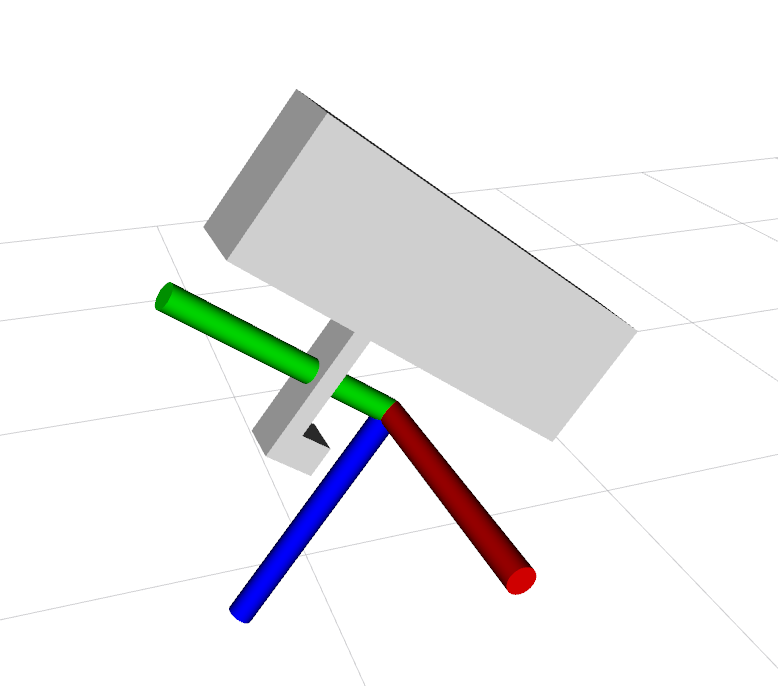
\includegraphics[width=\linewidth]{figures/panda_grasp_1.png}
    \caption{Good frame placement.}
\end{subfigure}%
\hfill
\caption{The location of the gripper frame used to compute the target reaching cost for manipulation can play a big role in finding a successful manipulation strategy.}\label{fig:frame_placement}
\end{figure}

In future work we would like to alleviate these issues by developing solutions that don't depend on more sampling and rather simplify cost engineering in a way to make it less sensitive to tuning and more generalizable across tasks. One way of achieving this goal would be to use a perception system to extract candidate interaction points and orientations from sensor data (as in~\cite{nagarajan2019grounded}), as an automated way of generating an ``interaction prior" in a continuous and real-time fashion. 

\subsection{Sim-to-real Gap}
Last but not least, particular care must be taken regarding the chosen physics engine used as a rollouts provider. Tuning is often required to reduce the compute time and allow for a longer prediction horizon. One simple way, also adopted in this work, is to increase the simulation step size at the cost of accuracy. This is in part compensated by the closed-loop nature of the control method that will reset the simulation to the newly observed robot state and therefore limit the simulation drift. Nowadays, there exists a plethora of physics engines that differ in algorithms, programming language and functionalities. A quantitative evaluation of the simulation accuracy and a comparative analysis is out of the scope of this work and recent reviews suggest that there isn't an obvious winner~\cite{collins2021review}. Nevertheless, when the task to solve is more complex, including contacts between more bodies and extends over a longer prediction horizon, we think that simulation fidelity can substantially improve the controller performance and therefore should be further investigated. 
